% !TeX root = ../main.tex

\chapter{水下穿戴式感知增强系统设计}
潜水员在深海环境中工作面临着复杂的水下环境。为了帮助潜水员在水下作业时提供全面的外界感知,
本章设计了一套具备水下环境三维可视化渲染功能的可穿戴系统。
该系统基于水下图像增强算法和三维重建技术,能够高质量恢复水下图像,并结合3D高斯泼溅技术渲染出逼真的水下场景。
通过嵌入手势识别技术,系统实现了人机交互功能,为潜水员在复杂场景下提供直观的视觉增强和操作便利性。

\section{设计目标与需求分析}
\subsection{系统设计目标}

在设计水下穿戴式感知增强系统时,我们的首要目标是为潜水员提供一个能够在复杂水下环境中增强感知能力的工具。具体而言,该系统的设计目标包括以下几个方面:

1. **增强水下视觉感知**:通过集成先进的水下图像增强算法和三维重建技术,系统能够在水下环境中提供高质量的视觉信息。这不仅包括清晰的图像和视频,还包括逼真的三维场景渲染,以帮助潜水员更好地理解周围环境。

2. **实时数据处理与反馈**:系统需要具备强大的实时数据处理能力,能够在潜水员移动时快速处理和反馈环境信息。这要求嵌入式处理器具备高效的计算能力,以支持复杂的图像处理和三维渲染任务。

3. **可靠的水下操作**:系统的所有组件,包括相机、显示器和处理器,必须在水下高压和腐蚀性环境中保持稳定运行。为此,系统设计了防水和抗压的外壳结构,确保设备在深海环境中的可靠性。

4. **直观的人机交互**:通过手势识别技术,系统实现了自然的人机交互方式。潜水员可以通过简单的手势与系统进行交互,避免了传统物理按键在水下操作的不便。

5. **长时间续航能力**:考虑到潜水作业的持续时间,系统设计了高容量的电源模块,确保设备能够长时间稳定运行。同时,系统的功耗管理机制能够在高性能和低功耗之间实现动态平衡。

6. **模块化设计与可扩展性**:系统采用模块化设计,便于后续的功能扩展和硬件升级。无论是增加新的传感器模块,还是升级现有的处理器和显示器,系统都能够灵活适应。

\subsection{系统需求分析}

为了实现上述设计目标,系统在功能和性能上需要满足以下具体需求:

1. **图像与视频采集需求**:
   - 系统需要配备高分辨率的RGB-D相机,能够在不同光照条件下采集清晰的彩色图像和深度信息。
   - 相机的帧率应达到90fps,以确保实时性和流畅性。

2. **数据处理与存储需求**:
   - 嵌入式处理器需要具备强大的计算能力,支持深度学习推理和复杂的图像处理算法。
   - 系统应具备足够的存储空间,用于存储采集的图像数据和处理结果。

3. **显示与交互需求**:
   - 头戴式显示器需要具备高清分辨率,确保潜水员能够清晰查看图像和三维场景。
   - 系统应支持手势识别功能,提供直观的交互方式。

4. **防水与结构强度需求**:
   - 所有设备必须具备IP68级别的防水性能,能够在50米深度下正常工作。
   - 系统的外壳材料需具备高强度和抗腐蚀性,确保在海水环境中的长期使用。

5. **电源与续航需求**:
   - 系统需配备高容量锂电池,支持长时间的潜水作业。
   - 电源模块应具备过载保护和充电功能,确保安全性和便利性。

6. **环境适应性需求**:
   - 系统需具备良好的散热性能,防止设备在高负荷运行时过热。
   - 设计气压平衡机制,防止外界压力变化导致设备变形或密封失效。

7. **扩展性与兼容性需求**:
   - 系统设计应具备良好的扩展性,支持未来的硬件升级和功能扩展。
   - 硬件和软件接口需具备良好的兼容性,支持与其他设备和系统的集成。

通过满足这些需求,水下穿戴式感知增强系统将能够为潜水员提供一个可靠、高效且直观的工具,帮助他们在复杂的水下环境中进行作业。系统的设计不仅关注当前的技术实现,还为未来的技术进步和应用扩展提供了可能性。



\section{系统平台搭建} 
\subsection{硬件选型与系统架构}
本章设计的水下穿戴式感知增强系统主要由相机、头戴式显示器、嵌入式处理器以及电源模块组成,
如图\ref{img:system}所示。
\begin{figure}
    \centering
    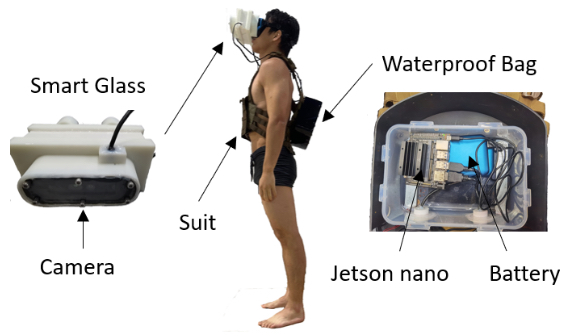
\includegraphics[width=0.8\textwidth]{figures/ch5/architecture of system.jpg}
    \caption{水下穿戴式感知增强系统组成}
    \label{img:system}
\end{figure}


(1)相机:
选用Realsense D455作为主摄像头,具备RGB-D功能,能够同时采集高分辨率的彩色图像和深度信息。
该相机封装于丙烯酸材料制成的防水外壳内,保证在水下高压环境中的稳定性。
其分辨率达到1280x720,帧率可达90fps,能够实时提供清晰的环境信息。

(2)头戴式显示器:
头显采用5英寸显示屏,分辨率为1920x1080像素,确保潜水员可以清晰地查看相机捕获的图像和三维场景。
显示器通过微型HDMI与嵌入式计算机连接,外壳基于谷歌VR纸板设计并用环氧树脂进行防水处理,确保水下使用的可靠性。

(3)嵌入式处理器:
选用NVIDIA Jetson Orin Nano作为核心计算单元,具备强大的边缘计算能力。
其GPU架构为Ampere,拥有48 Tensor Cores,支持深度学习推理加速,能够实时处理去噪扩散模型和3D高斯泼溅算法所需的计算任务。
处理器支持10W和20W两种功耗模式,结合自适应供电机制,确保系统在高性能和低功耗之间平衡。

(4)电源模块:
系统采用高容量锂电池组,容量为20,000mAh,输出电压为12V,满足Jetson Orin Nano的电力需求。
电池组集成于防水背包中,通过防水接头连接处理器,具备充电和过载保护功能,确保长时间潜水作业的稳定运行。

\subsection{防水与机械设计}
在水下环境中,设备的防水性和结构强度是决定系统可靠性的重要因素。
本系统设计了一套集成化的防水舱体与结构优化方案:

(1)防水背包:
\begin{figure}[h]
    \centering
    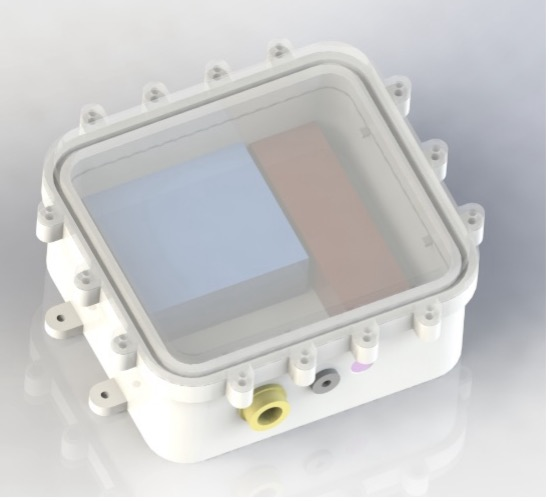
\includegraphics[width=0.6\textwidth]{figures/ch5/bag.jpg}
    \caption{防水背包设计}
    \label{img:bag}
\end{figure}

如图\ref{img:bag}所示,背包外壳采用高强度工程塑料,表面涂覆抗腐蚀层。
密封方式采用多层硅胶垫片与不锈钢紧固件结合,确保防水等级达到IP68。
出线采用专用防水接头和穿线螺丝,接口部分涂覆环氧树脂胶,进一步增强防水性能。
为了实现浮力与重力平衡,背包底部嵌入两块承重铁块。

(2)穿戴式头显设计:
如图\ref{img:camera}所示,
Realsense D455相机安装于透明丙烯酸外壳内,壳体经过高压测试,能够在50米深度下正常工作。
外壳通过双层O型圈进行密封,确保在水压变化下不发生渗漏。
\begin{figure}[ht]
    \centering
    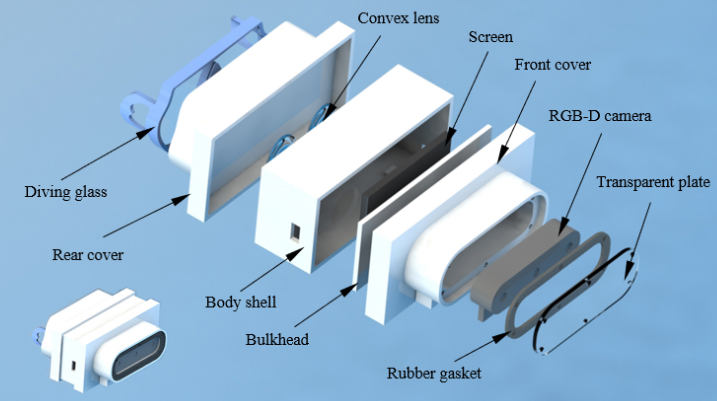
\includegraphics[width=0.85\textwidth]{figures/ch5/headscreen.jpg}
    \caption{相机防护设计}
    \label{img:camera}
\end{figure}

头显的镜片采用聚碳酸酯材料,经过耐冲击和防刮擦处理。
镜框与镜片之间采用液态硅胶封装技术,边缘增加防护垫圈。

(3)散热与气压平衡
嵌入式计算单元的热量通过金属导热片传递至外壳,并通过水体进行散热。
防水舱体内部设计了气压平衡阀,防止外界压力导致设备变形或密封失效。

另外,各部件之间通过防水接头连接,整体结构紧凑,确保在水下环境中的稳定运行。

\section{整体功能设计}
本章设计的水下穿戴式感知系统主要由穿戴式夹克组成,其上集成了防水舱体和水下虚拟现实头显。
该系统能够将直接捕捉视觉数据反馈至头戴式显示器,
通过 Jeston Orin 处理器实时渲染提前处理好的水下三维场景,
并结合手势识别技术实现在水下的全面的交互交互。

\subsection{图像增强与三维重建}
本文提出的水下可穿戴感知增强系统,通过整合第三章提出的水下图像增强算法和第四章的三维重建技术,为潜水员提供了高质量、逼真的水下三维场景。
系统整体设计如图 \ref{img:function} 所示,包含从数据采集到模型部署的全流程解决方案。
\begin{figure}[ht]
    \centering
    \includegraphics[width=0.97\textwidth]{figures/ch5/function.pdf}
    \caption{系统功能设计}
    \label{img:function}
\end{figure}

系统首先需要采集目标水下场景的多视角图像数据。为了确保采集的全面性和灵活性,可以利用自主水下机器人(AUV)或远程操作机器人(ROV)围绕目标区域进行视频拍摄。
对于采集到的视频数据,采用抽帧方法获取连续的图像序列。然而,受制于水下环境的特性(如光散射、颜色失真、低对比度等),原始水下图像通常存在模糊、色偏和细节丢失问题,这为后续的特征点匹配和点云生成带来了显著挑战。
为解决这些问题,系统集成了基于去噪扩散模型的水下图像恢复算法。该算法能够有效修复水下图像质量,通过去除噪声、校正颜色偏差、增强对比度等处理步骤,生成语义信息丰富且高质量的水下图像。
这一处理不仅提升了图像的视觉质量,也为后续的三维重建提供了更为可靠的数据基础。

在获得增强后的高质量水下图像后,系统利用结构化运动(SfM)技术完成初步三维重建。
SfM 技术的核心优势在于,即便在无相机内部参数的情况下,也能通过 2D 图像之间的特征点匹配,推断出相机的位姿以及场景的初步三维点云数据。
系统将处理好的水下图像输入 SfM 算法,通过精确的特征点匹配生成初始三维点云数据及对应的相机位姿。
这些点云数据往往较为稀疏,难以直接支持高质量三维模型的构建。
为此,系统引入基于算法 \ref{eq:knn} 的点云补充策略,通过邻域搜索对稀疏点云进行插值与补全,生成更为密集的点云数据。
这一过程为后续的三维高斯模型训练提供了丰富的数据支撑,避免了初始化阶段因数据不足导致的不稳定性。

在点云数据准备充分的情况下,系统利用基于 3D 高斯泼溅的三维重建算法完成水下场景的训练。
训练过程可以在地面端进行,通过高性能计算设备对三维模型进行迭代优化,以确保模型能够精确还原水下场景的细节与结构。
训练好的三维模型可以部署到轻量级的嵌入式设备(Jetson Orin Nano)中,实现实时场景预览显示。

\subsection{用户交互与控制}
本文的3D高斯渲染可视化通过 SIBR gaussianViewer 软件实现最后训练结果的三维实时预览,
该软件支持FPS第一人称导航视角控制方式来进行三维场景的浏览,
可以通过六个方向键位来控制视角的上下左右前后的移动以及六个旋转键位来控制对应的旋转。

为了提高潜水员在水下环境中的操作便利性,系统设计了一套基于手势识别的用户交互方案,
传统的基于物理按键的交互在水下受防水结构限制导致操作不便,因此本文基于手势识别算法设计了一套水下交互指令,
潜水员可以通过设定的手势指令完成与三维可视化场景预览界面的交互。

RoboChatGest\cite{robochatgest}开发了一个简单的交互框架,潜水员可以使用一套直观而有意义的手势与机器人进行交互。
为了设计简单而富有表现力的语言规则,本文选择了RoboChatGest中的一个视觉上更独特和直观的小手势集作为最后的交互手势原语,如表\ref{tab:chatgest}所示。
% \begin{figure}
%     \centering
%     \includegraphics[width=0.95\textwidth]{figures/ch5/chatgest.jpg}
%     \caption{手势识别原语}
%     \label{img:chatgest}
% \end{figure}


\begin{table}[ht]
\centering
\begin{tabular}{|c|c|c|c|c|c|c|c|c|c|}
\hline
\textbf{0} & \textbf{1} & \textbf{2} & \textbf{3} & \textbf{4} & \textbf{5} & \textbf{left} & \textbf{right} & \textbf{pic} & \textbf{ok} \\ \hline
\adjustbox{valign=c}{\includegraphics[width=1cm]{figures/ch5/res/d0.jpg}} & 
\adjustbox{valign=c}{\includegraphics[width=1cm]{figures/ch5/res/d1.jpg}} & 
\adjustbox{valign=c}{\includegraphics[width=1cm]{figures/ch5/res/d2.jpg}} & 
\adjustbox{valign=c}{\includegraphics[width=1cm]{figures/ch5/res/d3.jpg}} & 
\adjustbox{valign=c}{\includegraphics[width=1cm]{figures/ch5/res/d4.jpg}} & 
\adjustbox{valign=c}{\includegraphics[width=1cm]{figures/ch5/res/d5.jpg}} & 
\adjustbox{valign=c}{\includegraphics[width=1cm]{figures/ch5/res/d6.jpg}} & 
\adjustbox{valign=c}{\includegraphics[width=1cm]{figures/ch5/res/d7.jpg}} & 
\adjustbox{valign=c}{\includegraphics[width=1cm]{figures/ch5/res/d8.jpg}} & 
\adjustbox{valign=c}{\includegraphics[width=1cm]{figures/ch5/res/d9.jpg}} \\ \hline
\adjustbox{valign=c}{\includegraphics[width=1cm]{figures/ch5/res/u0.jpg}} & 
\adjustbox{valign=c}{\includegraphics[width=1cm]{figures/ch5/res/u1.jpg}} & 
\adjustbox{valign=c}{\includegraphics[width=1cm]{figures/ch5/res/u2.jpg}} & 
\adjustbox{valign=c}{\includegraphics[width=1cm]{figures/ch5/res/u3.jpg}} & 
\adjustbox{valign=c}{\includegraphics[width=1cm]{figures/ch5/res/u4.jpg}} & 
\adjustbox{valign=c}{\includegraphics[width=1cm]{figures/ch5/res/u5.jpg}} & 
\adjustbox{valign=c}{\includegraphics[width=1cm]{figures/ch5/res/u6.jpg}} & 
\adjustbox{valign=c}{\includegraphics[width=1cm]{figures/ch5/res/u7.jpg}} & 
\adjustbox{valign=c}{\includegraphics[width=1cm]{figures/ch5/res/u8.jpg}} & 
\adjustbox{valign=c}{\includegraphics[width=1cm]{figures/ch5/res/u9.jpg}} \\ \hline
\end{tabular}
\caption{手势识别原语}
\label{tab:chatgest}
\end{table}



如表\ref{tab:instruction}所示,本文基于上述的十个手势原语的各种组合设计了一个简单而强大的手势交互指令,潜水员可以通过这些手势与系统进行交互。
\begin{table}[h!]
\centering
\begin{tabular}{|c|c|c|c|c|}
\hline
指令 & 
键盘控制 &
左手手势 & 
右手手势 & 
token \\ 
\hline

开始 & 
- &
\adjustbox{valign=c}{\includegraphics[width=0.07\linewidth]{figures/ch5/res/d9.jpg}} & 
\adjustbox{valign=c}{\includegraphics[width=0.07\linewidth]{figures/ch5/res/d9.jpg}} & 
\{ok, ok\} \\ 
\hline

停止 & 
- &
\adjustbox{valign=c}{\includegraphics[width=0.07\linewidth]{figures/ch5/res/d0.jpg}} & 
\adjustbox{valign=c}{\includegraphics[width=0.07\linewidth]{figures/ch5/res/d0.jpg}} & 
\{0, 0\} \\ 
\hline

向前移动 &
W &
\adjustbox{valign=c}{\includegraphics[width=0.07\linewidth]{figures/ch5/res/d5.jpg}} &
\adjustbox{valign=c}{\includegraphics[width=0.07\linewidth]{figures/ch5/res/d1.jpg}} &
\{5, 1\} \\
\hline

向后移动 &
S &
\adjustbox{valign=c}{\includegraphics[width=0.07\linewidth]{figures/ch5/res/d5.jpg}} &
\adjustbox{valign=c}{\includegraphics[width=0.07\linewidth]{figures/ch5/res/d2.jpg}} &
\{5, 2\} \\
\hline

向左移动 & 
A &
\adjustbox{valign=c}{\includegraphics[width=0.07\linewidth]{figures/ch5/res/d5.jpg}} &
\adjustbox{valign=c}{\includegraphics[width=0.07\linewidth]{figures/ch5/res/d6.jpg}} &
\{5, left\} \\
\hline

向右移动 &
D &
\adjustbox{valign=c}{\includegraphics[width=0.07\linewidth]{figures/ch5/res/d5.jpg}} &
\adjustbox{valign=c}{\includegraphics[width=0.07\linewidth]{figures/ch5/res/d7.jpg}} &
\{5, right\} \\
\hline

向上移动 &
Q &
\adjustbox{valign=c}{\includegraphics[width=0.07\linewidth]{figures/ch5/res/d5.jpg}} &
\adjustbox{valign=c}{\includegraphics[width=0.07\linewidth]{figures/ch5/res/d3.jpg}} &
\{5, 3\} \\
\hline

向下移动 &
E &
\adjustbox{valign=c}{\includegraphics[width=0.07\linewidth]{figures/ch5/res/d5.jpg}} &
\adjustbox{valign=c}{\includegraphics[width=0.07\linewidth]{figures/ch5/res/d4.jpg}} &
\{5, 4\} \\
\hline

向上旋转(视角上移) &
I &
\adjustbox{valign=c}{\includegraphics[width=0.07\linewidth]{figures/ch5/res/d8.jpg}} &
\adjustbox{valign=c}{\includegraphics[width=0.07\linewidth]{figures/ch5/res/d1.jpg}} &
\{pic, 1\} \\
\hline

向下旋转(视角下移) &
K &
\adjustbox{valign=c}{\includegraphics[width=0.07\linewidth]{figures/ch5/res/d8.jpg}} &
\adjustbox{valign=c}{\includegraphics[width=0.07\linewidth]{figures/ch5/res/d2.jpg}} &
\{pic, 2\} \\
\hline

向左旋转(视角左移) &
J &
\adjustbox{valign=c}{\includegraphics[width=0.07\linewidth]{figures/ch5/res/d8.jpg}} &
\adjustbox{valign=c}{\includegraphics[width=0.07\linewidth]{figures/ch5/res/d6.jpg}} &
\{pic, left\} \\
\hline

向右旋转(视角右移) &
L &
\adjustbox{valign=c}{\includegraphics[width=0.07\linewidth]{figures/ch5/res/d8.jpg}} &
\adjustbox{valign=c}{\includegraphics[width=0.07\linewidth]{figures/ch5/res/d7.jpg}} &
\{pic, right\} \\
\hline

顺时针旋转(视角顺时针倾斜) &
O &
\adjustbox{valign=c}{\includegraphics[width=0.07\linewidth]{figures/ch5/res/d8.jpg}} &
\adjustbox{valign=c}{\includegraphics[width=0.07\linewidth]{figures/ch5/res/d3.jpg}} &
\{pic, 3\} \\
\hline

逆时针旋转(视角逆时针倾斜) &
U &
\adjustbox{valign=c}{\includegraphics[width=0.07\linewidth]{figures/ch5/res/d8.jpg}} &
\adjustbox{valign=c}{\includegraphics[width=0.07\linewidth]{figures/ch5/res/d4.jpg}} &
\{pic, 4\} \\
\hline

\end{tabular}
\caption{SIBR gaussianViewer 交互指令映射表}
\label{tab:instruction}
\end{table}


\section{系统实践与评估}

\subsection{实验环境}
\subsection{评估方案}
\subsection{功能测试}


\section{本章小结}














